\documentclass[10pt, twocolumn, twoside]{article}
\usepackage[top=1.2in, bottom=0.7in, left=0.7in, right=0.7in]{geometry}
\usepackage{amsmath}
\usepackage{amsthm}
\usepackage{amssymb}
\usepackage{placeins}
\usepackage{marvosym}
\usepackage[usenames,dvipsnames,table]{xcolor}
\usepackage{colortbl}
\usepackage{booktabs}
\usepackage{graphicx}
\usepackage{framed}
\usepackage{setspace}
\usepackage{xspace}
\usepackage[labelfont=bf]{caption}
\usepackage{verbatim}
\usepackage{paralist}
\usepackage{algorithm}
\usepackage{algpseudocode}
\usepackage{wrapfig}
\usepackage[font=footnotesize,labelfont=bf,justification=justified,singlelinecheck=false]{caption}
\usepackage{titlesec}
\usepackage{natbib}
\usepackage{longtable}
\usepackage{tabularx}
\usepackage{tabulary}
\usepackage{multirow}
\usepackage{lipsum}
\usepackage{mathpazo}
\usepackage{authblk}
\usepackage{nameref}
\usepackage{cancel}
\usepackage{commath}
\usepackage{xspace}
\usepackage{dsfont}
\usepackage{cuted}
\usepackage{fancyhdr}
\usepackage{hyperref}
\usepackage{longtable}
\usepackage{lineno}
\linenumbers
\setcounter{secnumdepth}{0}

% bib
\setcitestyle{aysep={}}
\renewcommand{\bibsection}{\section*{\normalsize References}}
\setlength{\bibsep}{0pt plus 0.3ex}

% hyperref setup
\hypersetup{
  colorlinks = true,
  linkcolor = {blue},
  citecolor = {blue}
}

% distance between columns
\setlength{\columnsep}{6ex}

% section rules
\titleformat{\paragraph}[runin]
{\normalfont\itshape}
{\theparagraph}{}{\noindent}[.---]

\titlespacing{\paragraph}{0pt}{3.25ex plus 1ex minus .2ex}{0em}

\titleformat{\section}
  {\centering\scshape}{\thesection}{1em}{}

\titleformat{\subsection}
  {\centering\itshape}{\thesubsection}{1em}{}

% bibliography settings

% other stuff?
\setlength\bigstrutjot{3pt}
\makeatletter
\newlength\mylena
\newlength\mylenb
\newcommand\mystrut[1][2]{%
    \setlength\mylena{#1\ht\@arstrutbox}%
    \setlength\mylenb{#1\dp\@arstrutbox}%
    \rule[\mylenb]{0pt}{\mylena}}
\makeatother

%%redefine longtable
%\makeatletter
%\let\oldlt\longtable
%\let\endoldlt\endlongtable
%\def\longtable{\@ifnextchar[\longtable@i \longtable@ii}
%\def\longtable@i[#1]{\begin{figure}[t]
%\onecolumn
%\begin{minipage}{0.5\textwidth}
%\oldlt[#1]
%}
%\def\longtable@ii{\begin{figure}[t]
%\onecolumn
%\begin{minipage}{0.5\textwidth}
%\oldlt
%}
%\def\endlongtable{\endoldlt
%\end{minipage}
%\twocolumn
%\end{figure}}
%\makeatother

% header
\pagestyle{fancy}
\fancyhf{}
\fancyhead[RO,LE]{\thepage}
\fancyhead[C]{\scshape VETR ET AL. --- BAYESIAN MULTIVARIATE BROWNIAN MOTION}

% Title %

\title{\vspace{-2.5cm}Bayesian Phylogenetics Under Multivariate Brownian Motion}
\author[$1,2,3$]{Nikolai G. Vetr}
\author[$2$]{Michael R. May}
\author[$2$]{Brian R. Moore}
\author[$1,*$]{Timothy D. Weaver}

\affil[$1$]{\small\itshape Department of Anthropology, University of California, Davis, Young Hall, Davis, CA 95616, USA;}
\affil[$2$]{\small\itshape Center for Population Biology, University of California, Davis, Storer Hall, Davis, CA 95616, USA;}
\affil[$3$]{\small\itshape Department of Pathology, Stanford University, 300 Pasteur Way, Stanford, CA  94305, USA;}
\affil[$*$]{\small\itshape E-mail: tdweaver@ucdavis.edu}
\date{}

\begin{document}

\maketitle{}

% Abstract %

\begin{strip}
\begin{makebox}[\textwidth][c]{
  \begin{minipage}{0.9\textwidth}
  \small
  \paragraph{Abstract}\vspace{-1cm}
  The field of statistical phylogenetics has progressed tremendously in recent decades. However, the development and application of molecular evolutionary models stand in stark contrast to limited adoption of corresponding models of morphological evolution. Given the nature of data primarily available to paleontologists and paleoanthropologists — shapes and sizes of bones and teeth — insufficient exploration of morphological models has impeded statistical inference of phylogeny among fossil taxa too old for the preservation of ancient DNA. Here, we present and perform inference under a stochastic multivariate Brownian diffusion model informed by quantitative genetics to describe the evolution of continuous traits. Unlike previous work, our model explicitly accommodates non-independence among traits, which may more realistically reflect biological phenomena such as pleiotropy and developmental integration. We then explore the statistical behavior of this model through analysis of simulated data and evaluate its performance with respect to retrieving simulating phylogenetic model parameters, with particular focus on tree topology. Finally, we apply our method to an empirical dataset consisting of 57 craniometric measurements collected by William W. Howells on a globally distributed set of modern human populations. Posterior distributions obtained from this analysis were consistent with accepted relationships in these groups. Several extensions of this model are also in development that will allow it to flexibly accommodate a wider range of data, such as polymorphic discrete morphological traits, and join it with molecular data to better shed light on evolutionary relationships linking both fossil and extant taxa. [Statistical Phylogenetics; Morphological Evolution; Bayesian Inference; Multivariate Brownian Motion]
  \end{minipage}
}
\end{makebox}
\end{strip}

%%%%%%%%%
% Intro %
%%%%%%%%%


\section{Introduction}

Statistical phylogenetics has undergone tremendous methodological progress in recent decades \citep{hollandRiseStatisticalPhylogenetics2013}. Most efforts, however, have centered on the description and implementation of discrete-state continuous-time Markov chain (CTMC) models of nucleotide substitution, with comparatively little attention paid to the development of morphological evolutionary models. When genetic data are available, both paleontologists and neontologists can fit molecular phylogenetic models in their framework of choice to make inference of the phylogenetic relationships linking taxa of interest, as well as many other phylogenetic model parameters. But for inferring phylogeny, paleontologists can only make direct use of molecular phylogenetics insofar as they can obtain viable ancient DNA – degradation quickly limits the temporal depths from which taxa can be drawn \citep{collinsSurvivalOrganicMatter2002, allentoftHalflifeDNABone2012, pickrellNewHistoryGeography2014}. Past those limits, they must use morphology to infer phylogeny.

Methods for inferring phylogeny using morphological characters are limited \citep{hollandRiseStatisticalPhylogenetics2013, leeMorphologicalPhylogeneticsGenomic2015}. Currently, both model-based and heuristic methods are commonly used. The former rely on mathematically explicit descriptions of evolutionary process and can be fitted in both Bayesian and Maximum Likelihood frameworks. For morphological characters, the most popular inference model is Lewis’ (\citeyear{lewisLikelihoodApproachEstimating2001}) Mk-model, which is the $k$-state generalization of the Jukes-Cantor (\citeyear{jukesEvolutionProteinMolecules1969}) model of nucleotide substitution (when $k$ = 4, the models are equivalent, as the state-space of DNA is 4. For discrete binaries – morphological traits that can be present or absent, large or small, and so on – $k$ = 2). Here, a discrete morphological trait changes state according to a continuous time Markov process where rate is independent of current state and waiting times between transitions are exponentially distributed. Rate heterogeneity between independent traits is straightforward to accommodate \citep{wrightModelingCharacterChange2016}. Further generalization can allow for non-independence between traits by specifying states as combinations of traits and unequal rates of change between those combinations, but this rapidly swells the state-space even for modest numbers of traits (e.g. 10 non-independent binaries will have $2^{10}$ possible states). Correctly fitting this model under maximum likelihood produces a point estimate of tree topology, branch lengths, and evolutionary model parameters that corresponds to the parameter values under which the observed data are most probable (the Maximum Likelihood Estimate, or MLE). Conversely, in a Bayesian framework one's target of inference is the entire joint posterior distribution of phylogenetic model parameters, often approximated with Markov chain Monte Carlo (MCMC).

However, morphological variation between groups is frequently not discrete, but continuous. While distances (e.g. Euclidean or Mahalanobis distances based on variation in the continuous characters) can easily be computed between sets of continuous characters, inference under the Mk-model \citep{lewisLikelihoodApproachEstimating2001} requires that we discretize any continuous observations. This discretization can be done in a variety of ways \citep{garcia-cruzCodingQuantitativeCharacter2006, thorpeCodingMorphometricCharacters1984} in part subject to researcher preference, with some methods discarding more phylogenetically relevant information than others \citep{brazeauProblematicCharacterCoding2011}. But even discrete characters collected at the outset may just be discretizing some fundamentally quantitative feature \citep{wiensCharacterAnalysisMorphological2001}, relying on a researcher’s present observations and prior experiences instead of an explicit algorithm run on the character alignment in its entirety. As such, we may desire statistical methods for inferring phylogeny that can make direct use of continuous characters without discretizing them.

Brownian motion represents a mathematically and computationally tractable description of continuous character change and can be shown with quantitative genetics and appeal to the central limit theorem to approximate a variety of evolutionary processes under a polygenic, additive model, including evolution at mutation-drift equilibrium, fluctuating selection, and constant directional selection \citep{hansenTranslatingMicroevolutionaryProcess1996, weaverNeutralTheoryEvolution2018a, harmonPhylogeneticComparativeMethods2018}. 

Briefly, consider that under polygenicity, continuous character values are binomially distributed, and when the number of loci underlying a polygenic trait is high, the normal approximation to the binomial holds (via the central limit theorem, as binomial random variables are sums of independent Bernoulli random variables, which have finite variance). Since the difference between two normal random variables is itself normal, a Brownian motion model (described in further detail below) can be a good approximation of an evolutionary process acting under the above conditions. First described empirically by Brown (\citeyear{brownXXVIIBriefAccount1828}) and mathematically by Einstein (\citeyear{einsteinInvestigationsTheoryBrownian1956}), it has enjoyed considerable attention in the context of phylogenetic comparative methods \citep{felsensteinPhylogeniesComparativeMethod1985}, where it is often contrasted with more parameter-rich Gaussian models, such as the Hansen model \citep{butlerPhylogeneticComparativeAnalysis2004, beaulieuModelingStabilizingSelection2012}, to better understand the evolutionary processes that structure morphological variation when the tree on which the characters evolved is assumed to be known. Recently, the statistical performance of a univariate Brownian motion model has been explored through simulation \citep{parins-fukuchiUseContinuousTraits2017}. Here, moderate numbers of independent continuous traits contained sufficient information to reliably retrieve the simulating tree’s topological structure under varying degrees of model misspecification, though as correlation between traits increased in the simulating model so too did error under the misspecified inference model.

As phenomena such as integration, pleiotropy, linkage disequilibrium, and correlated selection are likely to structure the evolution of continuous traits \citep{cheverudDevelopmentalIntegrationEvolution1996, youngEvolutionaryPersistencePhenotypic2006, mitteroeckerConceptualStatisticalRelationship2007, klingenbergMorphologicalIntegrationDevelopmental2008, klingenbergStudyingMorphologicalIntegration2014} across a variety of taxa \citep[e.g.][]{parsonsConstraintOpportunityGenetic2011, klingenbergDevelopmentalPlasticityMorphological2012, neauxBasicraniumFaceAssessing2018}, it may not always be safe to assume each trait to be an independent realization of some univariate Brownian motion process.  Moreover, explicitly working within a multivariate framework can also enable more nuanced reconstruction of both fossil (in the case of fragmentary remains – i.e. missing data) and ancestral phenotypes (e.g. see Appendix 2) and permit the direct investigation of correlated evolution between traits, integrated over phylogenetic uncertainty.

Here, we describe an approach for inferring phylogeny from continuous-character data under a multivariate Brownian diffusion model that allows them to evolve non-independently. Then, we explore the statistical performance of the model and the validity of its RevBayes \citep{hohnaRevBayesBayesianPhylogenetic2016a} implementation using a comprehensive simulation study. Finally, we apply the method to well-studied empirical dataset consisting of cranial measurements collected on extant human populations \citep{howellsCranialVariationMan1973, howellsSkullShapesMap1989, howellsWhoWhoSkulls1995}. 

\clearpage

\section{Materials and Methods}

\subsection{Simulating from the Model}

Univariate Brownian motion (uvBM) describes a stochastic process where displacements to the value of some continuous character are drawn from univariate normal distributions. When undirected, the means of these distributions are zero and their variances are equal to the product of two scalars, one representing the branch length $v_i$ over which evolution occurs and the other representing the rate of continuous character change, $\sigma^2$ (Figure \ref{fig:univBM}). Multivariate Brownian motion (mvBM) generalizes this process to multiple characters. Under mvBM, displacements to the values of some vector of $n$ continuous characters are drawn from multivariate normal distributions, with mean $(0_1,0_2,...0_n)$ and covariance matrix given as the element-wise product $\Sigma = v_iR$, where $R$ is a square, symmetric, positive-semidefinite covariance matrix describing the rates and correlations of evolutionary change, collectively known as the multivariate Brownian rate matrix. A univariate Brownian motion of multiple characters can be seen as a special case of mvBM where all off-diagonal elements of $R$ are constrained to be 0; conversely, non-zero off-diagonal elements specify non-independent character evolution. It is common to decompose $R$ into the matrix product $SCS$, where $S$ is a diagonal matrix of standard deviations (constrained to be $>0$) with elements $\{\sigma_1, \sigma_2, ... \sigma_n\}$ specifying the square root of the rates of evolution under mvBM, and $C$ is a correlation matrix specifying their nonindependence. As a correlation matrix, $C$'s diagonal elements are defined to be 1, its off-diagonal elements restricted to the range (-1,1), and the resulting square, symmetric matrix $C$ constrained to be positive-semidefinite. As the diagonal elements of $S$ increase, corresponding characters experience greater potential for evolution; as the off-diagonal elements of $C$ stray further from 0, corresponding pairs (or modules) of traits evolve in an increasingly correlated fashion.


Multivariate Brownian motion can also describe correlated character evolution on a phylogenetic tree. On a phylogeny, lineages multifurcate at internal nodes and continue on independent evolutionary trajectories –  displacements drawn on one lineage subsequent to multifurcation are independent of the states observed or displacements drawn at other lineages. From some starting (e.g. root) state, one can simulate along a branch by adding to that state a draw from a normal distribution whose variance is the aforementioned product. Upon reaching an internal node, character evolution along each daughter branch can be further simulated by additional independent displacements from separate normal distributions. Alternatively, to simulate a vector containing end states across all the tips (or internal nodes, positions along branches, etc.) of the phylogeny, one can make a single draw from a multivariate normal distribution whose mean is the state at the root and whose covariance matrix is the phylogenetic covariance matrix ($O$), with elements representing the shared evolutionary history of each pair of tips, or the sum of those branch lengths shared by each pair of tips stretching back to the root. Diagonal elements of the $O$ matrix are the height of corresponding tips above the root of the tree, as each tip shares the entirety of its evolutionary history with itself. For example, one can sample a vector of character data $x$ = $\{x_A, x_B, x_C\}$ for a single trait evolving under univariate Brownian motion with rate $\sigma^2$ on the tree depicted in Figure \ref{fig:simpleTree} by sampling from a multivariate normal distribution with mean $\{x_E, x_E, x_E\}$ and covariance matrix:

{\large\[\sigma^{2}P = \begin{bmatrix}
\sigma^{2}v_1 & 0 & 0 \\
0 & \sigma^{2}(v_4 + v_2) & \sigma^{2}v_4 \\
0 & \sigma^{2}v_4 & \sigma^{2}(v_4 + v_3) \\
\end{bmatrix}\]}

Conversely, multivariate Brownian motion (mvBM) generalizes the above process to multiple characters evolving non-independently. Instead of sampling from univariate normal distributions when simulating along branches, one samples from multivariate normal distributions whose means are a vector of zeros and whose covariance matrices are equal to the product of each scalar branch length and some covariance matrix representing the rates and correlations of evolution in a set of continuous characters (i.e., $R$). To simulate a vector $X$ containing states for all the characters across all the tips of the phylogeny, one can perform a similar pre-order traversal or, alternatively, take a single draw from a multivariate normal distribution whose mean is the state at the root and whose covariance matrix is given by the Kronecker product of $R$ and $O$. The elements of $X$ will be in order of sets of characters or tips, depending on the order in which one took the Kronecker product (for $R \otimes O$, elements of the $X$ are grouped first by characters and then by tips). The uvBM process, then, can be seen as a special case of mvBM where all the off-diagonal elements of $R$ are fixed to 0.

\subsection{Bayesian Inference}

We implement the above described multivariate Brownian motion process in a Bayesian framework to approximate the joint posterior distribution of phylogenetic and evolutionary model parameters, which may include S, C, and V, described above, given observed character data $X$. It is common to represent the phylogenetic covariance matrix $O$ as two distinct parameters: a discrete tree topology $\Psi$ and a vector of appropriately indexed branch lengths $V$. The joint posterior density of model parameters can then be described by 

{\[P(S, C, \Psi, V | X) \propto P(X | S, C, \Psi, V) P(S, C, \Psi, V)\]}

which states that this density is proportional to the product of the likelihood, a term that gives the plausibility of observing $X$ given parameter values, and the joint prior density, which represents our beliefs about those parameter values prior to observing data. Computation of the likelihood is described below, and prior densities can be specified through one's choice of prior distributions, which can in turn be influenced by external information or by a desire for regularization. The sensitivity of the results of an empirical analysis can and should be evaluated with respect to one's choice from a reasonable set of prior distributions. As a probability distribution, the integral of $P(S, C, \Psi, V | X)$ across its range must equal 1, so we may divide the right-hand side of the above expression by $P(X)$, also known as the marginal likelihood, which represent the probability of the data, X, averaged over the prior $P(S, C, \Psi, V)$. In practice, closed-form solutions of $P(X)$ are difficult to express, so we instead exploit the above expression of proportionality to sample values from the distribution $P(S, C, \Psi, V | X)$ in proportion to their density using MCMC.

\subsection{Data}

The vector of observations, $X$, is a $p$ $x$ $t$ vector of continuous characters, where $p$ represents the number of observed nodes in the tree and $t$ represents the number of observed characters corresponding to each node. This vector can be represented by a matrix of dimension $(p, t)$, analogous to a nucleotide or amino acid sequence alignment in molecular phylogenetics. The order in which one constructs the vector (grouping together observations either by node or trait) is arbitrary, but must correspond to the order in which one takes the Kronecker product described earlier. It is common to specify a model of geometric Brownian motion, where the element-wise log of some vector of continuous characters undergoes (untruncated) Brownian motion, rather than the real-valued continuous characters themselves. This implies a multiplicative epistasis at the underlying gene level and is often done to restrict trait evolution to positive values only, though they can still grow arbitrarily large. 

\subsection{Likelihood}
The likelihood function under multivariate Brownian motion is equivalent to the probability density function of the multivariate normal distribution described above, N$(\mu, R \otimes O)$, and evaluates to a number proportional to the probability of observing some vectorized continuous character alignment conditional on matrices $R$ and $O$. It is given by the expression

{\large\[|2\pi\Sigma|^{-\frac{1}{2}}e^{-\frac{1}{2}(x-\mu)^T\Sigma^{-1}(x-\mu)}\]}

where $x$ is the stacked vector of tip characters, $\mu$ is the state at the root (corresponding to node $E$ in the above tree), and $\Sigma = R \otimes O$.

Often, this root state is unobserved – we can attempt to infer its location and value by making strong assumptions regarding the rates of character change, by specifying a prior on the root state (including a point-mass prior, where the root state is known without uncertainty), or by marginalizing over all possible states at the root — in effect, specifying a uniform($-\infty, \infty$) prior on it, as we implicitly do for states along branches and at internal nodes. As normal distributions are symmetric, the Pulley Principle holds \citep{felsensteinEvolutionaryTreesGene1981} and the probability under Brownian motion of going from state $i$ to state $j$ is identical to the probability of going from state $j$ to state $i$. As a result, the computed likelihood is invariant to the placement of the root, and one can calculate an identical likelihood by re-rooting at any position of the tree. This allows us to perform inference under unrooted trees and root according to our criterion of choice later (e.g. along a branch leading to an outgroup or at a node we have specified an informative root-state prior on). In other words, the trees depicted in Figure \ref{fig:pulleyPrinciple} — with observed states corresponding to nodes $\{A, B, C\}$ and unobserved states to $\{D, E\}$ — have identical likelihoods.

A likelihood that marginalizes over all possible root states can be called a “restricted” likelihood (or sometimes a “residual” or “reduced” likelihood, \citealt{felsensteinInferringPhylogenies2004}). Conveniently, this also shrinks the space of possible trees we need to integrate over, equivalent to dropping any of the terminal nodes of our tree.

Repeatedly computing densities of high-dimensional multivariate normals is computationally expensive, so we may wish to re-express the likelihood as a product of univariate normal densities. This can be done by diagonalizing both the $O$ and $R$ matrices and propagating the appropriate transformations in the likelihood function to the vector of tip states. Two algorithms will serve our purposes here. The first exploits the structure of the phylogenetic covariance matrix, $O$, by performing a post-order traversal of its corresponding tree and iteratively pruning off and computing densities of contrasts between neighboring tips, replacing each internal node’s pair of daughter lineages with the conditional (on the values of its descendants) multivariate normal distribution of the state at that internal node (Figure \ref{fig:pruningAlgorithm}). This algorithm, also called a “pruning” or “peeling” algorithm, was first described in a phylogenetic context by Felsenstein \citeyear{felsensteinMaximumlikelihoodEstimationEvolutionary1973, felsensteinPhylogeniesComparativeMethod1985, felsensteinInferringPhylogenies2004}, though in itself is just a special case of the sum-product algorithm applied to trees \citep{hohnaProbabilisticGraphicalModel2014}. It is directly analogous to the identically named algorithm also developed by Felsenstein used to accelerate likelihood calculation under nucleotide substitution models. Implicit to it is the diagonalization of the $O$ matrix by some transformation matrix that pre- and post-multiplies it, i.e.

{\large\[Q = COC^T\]}

We can solve for $O$ and substitute $C^{-1}QC^{-T}$ in to the multivariate normal PDF above, and through simple linear algebraic manipulation move each of $C^{-1}$ and $C^{-T}$ to transform $x$ into $y$, leaving the diagonal $Q$ in place of $\Sigma$ (where the elements of $y$ correspond to the values of the contrasts, and the elements of $\Sigma$ to those contrasts' branch lengths; see Appendix 1 for further mathematical details). The result of this procedure is a phylogenetic covariance matrix $Q$ whose off-diagonal elements are 0, corresponding to variances of the transformed character vector $y$ (i.e. the independent contrasts). This transformation subtracts out the parameter of the model corresponding to the root state, so if performing inference with a 'known' root, one must either re-root the tree elsewhere, or else include the root state in the vector $X$, with corresponding elements in $O$ set to zero.

Implementing this algorithm – in effect, populating the $C$ matrix above, but in practice constructing $Q$ and $y$ directly – is straightforward. Starting with some alignment of continuous characters at the tips, find a pair of sister tips. In the rooted 3-tip above, we can use any pair, but let us choose $\{B,C\}$. Compute the difference of their character states ($x_B – x_C$; or alternatively $x_C - x_B$) and set it as the first element(s) of $y$. Set the sum of the branch lengths separating $(v_2 + v_3)$ as the first (diagonal) element of $Q$. Then, prune off the two terminal branches leading to $B$ and $C$, and at the previously internal node representing their most recent common ancestor construct a new, virtual tip whose value is the normal distribution conditional on the values of $B$ and $C$. As normal distributions are additive in variance, this has the effect of extending the branch length of that virtual tip by the variance of the conditional distribution, and settings its value as the conditional distribution’s mean. For some multivariate normal distribution with mean and covariance matrix partitioned as

{\large\[\mu = \begin{bmatrix}
\mu_1 \\
\mu_2 \\
\end{bmatrix} \
\Sigma = \begin{bmatrix}
\Sigma_{11} & \Sigma_{12}\\
\Sigma_{21} & \Sigma_{22}\\
\end{bmatrix}
\]}

and realizations partitioned as

{\large\[x = \begin{bmatrix}
x_1 \\
x_2 \\
\end{bmatrix}\]}

The distribution of $x_1$ conditional on observed value(s) $x_2$ is also multivariate normal, with mean and covariance:

{\large\[\mu_1' = \mu_1 + \Sigma_{12}\Sigma_{22}^{-1}(x_2-\mu_2)\]}

{\large\[\Sigma_{11}' = \Sigma_{11} - \Sigma_{12}\Sigma_{22}^{-1}\Sigma_{21}\]}

In the above example, taking $x_1 = x_D$, $x_2 = x_C$, $\mu_1 = \mu_2 = x_B$, and

{\large\[\Sigma = \begin{bmatrix}
v_2 & v_2\\
v_2 & v_2+v_3\\
\end{bmatrix}\]}

we can solve for $\mu'_1 = x_B + v_2(v_2 + v_3)^{-1}(x_C – x_B) = (x_Bv_3 + x_Cv_2) / (v_2 + v_3)$ and $\Sigma’_{11} = v_2 - v_2(v_2 + v_3)^{-1}v_2 = v_1v_2/(v_1 + v_2)$. These describe the conditional normal distribution of that ancestral node – we can add its variance to the length of its subtending branch, and set as the virtual node’s value its mean. This procedure can be repeated until all the branches have been pruned and one is left with a fully populated vector $y$ and matrix $Q$ (whose dimensions are all one less than those of the original $x$ and $O$, an effect of marginalizing over the unobserved root state), corresponding to $n – 1$ independent contrasts and their variances.

Through this decomposition and diagonalization of $O$, we transform our original $R \otimes O$ covariance matrix into a diagonal block matrix containing $n – 1$ scalar products of $R$ matrices, requiring us to still calculate $n – 1$ multivariate normal densities and ensuring that compute time for a single likelihood calculation is roughly linear with tip number. We can further improve efficiency by diagonalizing $R$ so that each of these multivariate normal densities is rewritten as the product of univariate normal densities. This can be done through many decompositions, but here we choose a Cholesky decomposition of $R$ so that $R = LIL^T$, where $L$ is the lower Cholesky factor of $R$ and $I$ is an identity matrix of appropriate dimension. Substituting this expression in for $R$, we can propagate $L^{-1}$ through to premultiply $x$, though we must also take care to divide each contrast’s density by the determinant of $R$ (see Appendix 1 for mathematical details). During inference this decomposition and transformation must be reapplied each time the rate matrix changes (e.g. a proposal is made to the rate matrix during MCMC), but otherwise if most proposal weight is on parameters other than the rate matrix, compute time becomes approximately linear with trait number, plus any overhead in having to keep track of these further “transformed” tip values. In the analyses that follow in RevBayes \citep{hohnaRevBayesBayesianPhylogenetic2016a}, we saw an approximately 40-fold reduction in compute time over using the pruning algorithm alone when conditioning on a particular rate matrix (for analyses of 128 characters, with more improvement under higher dimensionality and less under lower). This approach can also improve efficiency when sampling rate matrices, if $R$ or its subcomponents are parameterized through their Cholesky factor, as can often be the case when specifying an LKJ prior on the correlations of $R$.

\subsection{Priors}

The algorithms described above are independent of one's choice of prior, and can indeed be applied just as well in a Maximum Likelihood inferential framework. Nevertheless, working in a Bayesian framework requires that we specify prior distributions on all unobserved parameters of the model, both for the simulations and for the empirical analyses that follow. We describe these distributions below. In this context, priors can help us to specify our beliefs about model parameters, accommodate inferential uncertainty, and regularize inference away from singularities in the likelihood surface under more parameter-rich models (e.g. when attempting to infer ancestral states jointly with branch rates, instead of marginalizing over them).

For the two sets of simulation experiments described below, we specify two sets of priors. In the first, we place a pure-birth \citep{yuleMathematicalTheoryEvolution1925} prior on the tree and branch lengths with speciation rate ($\lambda$) = 1, and tree height given as a point-mass prior on the ground truth height of the tree on which the simulation was performed. Additionally, we placed a point-mass prior on the rate matrix equivalent to that used in simulation, as this initial experiment focused more on the informativeness of continuous characters on tree topology, independent of uncertainty in the rate matrix. This lets us best explore retrieval of the topology parameter under optimal inferential conditions.

For the empirical analysis, we specified a more diffuse prior on branch lengths and topology – specifically, a discrete uniform prior on topology, a log-uniform ($10^{-3}$, $10^2$) prior on tree length, and a flat Dirichlet prior on branch lengths. These were chosen to avoid “long-tree” problems identified elsewhere \citep{brownWhenTreesGrow2009}, though for this dataset we found the posterior distribution with respect to topology to be largely insensitive to branch length prior specification. In contrast to the ``strict morphological clock" used above, this corresponds to a relaxed clock where individual branch rates have more freedom to vary. Here, we once more used a point-mass prior on the rate matrix, fixed to the sample pooled-within-group phenotypic covariance matrix calculated from our dataset. 

In the final simulation experiment, we used the same priors as in the empirical analysis described above.

\subsection{MCMC}

Inference was done in a Bayesian framework using the statistical phylogenetics environment \textit{RevBayes} \citep{hohnaRevBayesBayesianPhylogenetic2016a}. The Metropolis-Hastings algorithm \citep{hastingsMonteCarloSampling1970} was used to sample from the joint posterior of our phylogenetic model parameters, given that model, priors, and simulated continuous character alignment. This machinery is fundamentally identical to that used for phylogenetic inference from nucleotide sequence data, as well as in other Bayesian inference problems. Preliminary runs with Metropolis coupling (3 heated + 1 cold chain) resulted in no improvement to MCMC mixing, so all subsequent analyses were uncoupled to save on compute costs. Longer chains were run initially to identify adequate sampling intensity; final analyses were run for 35,000,000 iterations, with the first 7,000,000 used to tune proposal mechanisms to ensure intermediate acceptance probabilities and subsequently discarded as burn-in. \textit{RevBayes} allows for flexible specification of MCMC proposals, so a variety were used (see example script in supplemental information), with approximately half the proposal weight given to moves on topology and half given to moves on branch lengths. Two independent chains were run for MCMC diagnostics and their output later concatenated for downstream analysis. To compare inference under the simulating model to inference under a misspecified model representing univariate Brownian motion, we further replicated all analyses with off-diagonals of the inference rate matrix set to 0.

\subsection{Simulations}

We performed a series of simulation experiments to explore the statistical performance of this model, simulating continuous character alignments evolving under multivariate Brownian motion on trees drawn from several sets of trees. These first simulations were performed on trees with 30 tips sampled from a pure-birth \citep{yuleMathematicalTheoryEvolution1925} distribution (i.e. extinction rate = 0) with speciation rate = 1, though the scale invariance of Brownian motion would permit any birth rate, so long as differences between tips were far enough above machine precision and branch length priors during inference placed sufficient density on appropriately long branches (e.g. if we sampled trees with incredibly low speciation rates but placed low prior probability on ``long" trees, we might be led astray). We then simulated sets of (2, 4, 8, 16, 32, 64, 128) characters on these trees using rate matrices of simple correlation structure – all diagonals were set to 1 and all off-diagonals were equal and set to either (0, 0.2, 0.4, 0.6, 0.8, 0.99) in order to explore the impact of the number of characters and the strength of character correlation on the phylogenetic informativeness of continuous character data. To explore the effects of improperly assuming that tip values are known without error (e.g. measurement, taphonomic, environmental, etc.), we further perturbed the state for each tip at each trait by an i.i.d. normal random variable with mean 0 and variance 0.5, equivalent to extending each terminal branch of the tree by $\frac{1}{2}$ and evolving the trait vector via Brownian motion under a rate matrix equal to the identity matrix. We performed equivalent analyses on the unperturbed character alignments as well as these further perturbed tips without explicitly accommodating the perturbation in our inference model. To average out the effects of simulation variance, we performed 500 replicate simulations for each combination of simulating model parameters (trait \#, correlation strength, and the P/A of noise). Analyses of these simulated datasets were done under two inference models -- one where the character evolution process was perfectly specified and we conditioned on the true, data-generating rate matrix, and one where we conditioned on the true trait-specific rates (the diagonal of the rate matrix) but falsely conditioned on a univariate Brownian motion, fixing all off-diagonals to 0.

A second set of simulation experiments explored performance under more ``empirically-realistic" simulation conditions and is described below. Simulating models here were parameterized using MCMC output from our empirical analysis, and we further explored finer-grained rate-matrix misspecification than merely performing inference under a univariate model when the simulating model was fully multivariate.

\subsection{MCMC Diagnostics}
%MDS plots, compare tree plots, CSF plots, ACSF plots, ASDSF plots,
Several diagnostic criteria were used to ensure MCMC health and identify pathology. Many MCMC diagnostics rely on visual inspection (e.g. marginal histograms, rank plots, and trace plots) which would have been onerous to evaluate across millions of possible parameter-parameterization combinations, so instead we evaluated performance according to less qualitative criteria. Specifically, using the \textit{CODA} package \citep{plummerCODAConvergenceDiagnosis2006} in R \citep{rcoreteamLanguageEnvironmentStatistical2013}, we computed effective sample sizes on the following values, requiring that each fall above 1,000: patristic distances between all of pairs of tips, Robinson-Foulds \citep[RF][]{robinsonComparisonPhylogeneticTrees1981} and Felsenstein-Kuhner (KF; \citeyear{kuhnerSimulationComparisonPhylogeny1994}) distances from the true, data-generating tree, the computed likelihood value, the posterior density, the tree length, and Colless’ Index. Additionally, we computed the squared correlation coefficients on between-chain nodal probabilities appearing at frequencies above 0.005 in either chain, requiring that they be $> 0.95$. MCMC analyses failing any of these criteria (approximately 5\% of total runs) were rerun with triple the total run length. Those that failed these longer runs (approximately 2\% of total runs) were excluded from the results and new simulated data analyzed to achieve precisely 500 replicates per condition.

\subsection{Output Analysis}

Having obtained MCMC output and evaluated chain health, we sought to evaluate inferential performance, largely through consideration of its aggregate ``frequentist properties" \citep[\textit{sensu}][]{huelsenbeckFrequentistPropertiesBayesian2004}. First, we constructed calibration curves (sometimes called “reliability” curves) for nodal probabilities falling within equally spaced bins of 0.1 width. This procedure is commonplace in the machine learning literature when evaluating probabilistic classification algorithms, but phylogenetically has seen infrequent application. Specifically, we calculated the frequency with which a bipartition with probability falling in some bin was present in the true, data-generating tree, averaged across analyses. Perfect calibration would see observed frequency match inferred posterior probability, with plotted points falling along the 1:1 line, indicating that nodal probabilities are trustworthy and that the inference machinery is working correctly, conditional on the model being well-specified. Underconfidence would see true frequencies greater than posterior probabilities; overconfidence less. We examined nodal probabilities because data uninformativeness and the breadth of tree-space resulted in so diffuse a joint posterior that posterior probabilities for particular topologies were very small and unstable (e.g. the MAP tree was sampled at most a small handful of times, even with 128 characters). As the inference model grows increasingly misspecified, we expect to see greater and greater deviation from the state of perfect calibration.

Next, we evaluated how precisely tree topology could be retrieved. Traditional methods of doing so – e.g. computing distances of the true tree from some summary tree – could not be used because the data were so uninformative as to also compromise the stability of those summaries (using more than 128 traits would result in more stable summary trees, but may represent unrealistic sample sizes for data collection, especially given the need to integrate over rate matrices). Furthermore, summary trees – while useful for visualization – are not the target of Bayesian inference, whose interests instead are in the entirety of the joint posterior distribution of model parameters. Instead, we constructed a plot we have named the “Cumulative Average Resolution” (CAR) curve. Essentially, it compares across sets of analyses the average number of bipartitions that occur above some threshold probability. This corresponds to the number of nodes resolved in a consensus tree with of some probability cutoff (e.g. in the majority-rule consensus tree, that cutoff is 0.5; this is also where we start the CAR curve, as lower thresholds permit the inclusion of incompatible nodes). Examining the height and shape of the curve gives a sense of the typical informativeness of some quantity of data produced by an evolutionary model when performing inference under that or some other model. The curve resembles a staircase for a single analysis, but averaging across analyses we see greater and greater smoothness.


\subsection{Empirical Analyses}

Having explored the model through these initial simulations, we fit phylogenetic multivariate Brownian motion to an empirical dataset comprising linear craniometric measurements. These consisted of 57 linear distances between anatomical locations measured on 2,524 individuals identified as male or female by William W. Howells \citeyear{howellsCranialVariationMan1973, howellsSkullShapesMap1989, howellsWhoWhoSkulls1995} on crania drawn from a globally distributed sample of 30 modern human populations (Table \ref{tab:howellsDataComposition}). We chose this dataset because it is publicly available, well-known, and is often used to estimate tree-like population structure among modern humans, both by Howells but also more recently \citep[e.g.][]{rosemanRandomGeneticDrift2016}. Conditioning on tree structure without reticulation introduces some misspecification, however; future work to extend the model and incorporate reticulation between lineages in a joint inferential framework is ongoing \citep[following e.g.][]{pickrellInferencePopulationSplits2012}. In these analyses we conditioned on a rate matrix equivalent to the maximum likelihood estimate (MLE) of the pooled within-group phenotypic covariance matrix (P), adopting Cheverud’s conjecture \citep{cheverudDevelopmentalIntegrationEvolution1996, roffEstimationGeneticCorrelations1995, reuschQuantitativeGeneticsDung1998, waittGeneticPhenotypicCorrelations1998, revellPhylogeneticApproachDetermining2007} of proportionality between P and the additive genetic covariance matrix (G), which would in quantitative genetics dictate the availability of morphological change under several evolutionary models, but most commonly assumed to correspond to neutrality \citep{landeNaturalSelectionRandom1976, landeQuantitativeGeneticAnalysis1979, felsensteinPhylogeniesQuantitativeCharacters1988a}. The P matrix generally reflects mild-to-moderate non-independence between traits, with off-diagonals of its underlying correlation matrix having a middle 95th percentile interval of (-0.22, 0.69). These assumptions seem reasonable given that Cheverud’s conjecture has recently been confirmed for a small subset of human phenotypes \citep{sodiniComparisonGenotypicPhenotypic2018} and observed differences in the cranium between Neandertals and modern humans seem consistent with neutral evolutionary process \citep{weaverWereNeandertalModern2007, weaverUnconstrainedCranialEvolution2015}. Concentrating the rate matrix’ probability on a single point mass dramatically shrinks the free parameter space of the model and allows branch lengths to be interpretable in units of average within-population differentiation. This ``empirical Bayesian" approach is comparable to treating individuals as tips, constraining the monophyly of designated populations, and assuming star-like pedigree structures within populations of height one. To minimize the effects of sexual dimorphism, we performed independent analyses of individuals identified male and female by Howells. 

As rates of Brownian motion between lineages were thought unlikely to be constant throughout the tree, we specified a more diffuse prior on branch lengths and topology – specifically, a discrete uniform prior on topology, a log-uniform ($10^{-3}$, $10^2$) prior on tree length, and a flat Dirichlet prior on branch lengths. These were chosen to avoid “long-tree” problems identified elsewhere \citep{brownWhenTreesGrow2009}, though for this dataset we found the posterior distribution with respect to topology to be largely insensitive to branch length prior specification. These would allow for scalar variation in the rate matrix throughout the tree, but not variation in the correlation structure or relative rates of particular traits, though extending the model by either sampling states at internal nodes to numerically integrate over augmented likelihoods or using the modification described by Caetano and Harmon (\citeyear{caetanoEstimatingCorrelatedRates2019}) would permit variation in the structure of the rate matrix itself and better reflect our understanding of the instability of P \citep{fischerPlasticityEvolutionCorrelated2016} and G \citep{arnoldUnderstandingEvolutionStability2008}.

Maximum Clade Credibility Trees from these two analyses are presented in Figure \ref{fig:mccCophylo}. Specifically, these conditioned on a model of arithmetic Brownian motion, where the particles movement is on the scale of the raw distances themselves, without log-transform, to better reflect the additive nature of genetic variation. A separate analysis using a geometric Brownian motion model found inferred tree topologies almost entirely insensitive to flexibility in this respect, with bipartition probabilities in the compare-trees plot falling very close to the 1-to-1 line (Figure \ref{sensitivitySexGeom})

\subsection{Further Simulations}

To explore the reliability of these inferences, we performed a subsequent simulation study parametrized with an eye towards biological realism. Here, we simulated according to a multivariate Brownian motion process sets of 2, 4, 8, 16, 32, and 57 characters, and performed inference under the priors described for the empirical analyses described above and a rate matrix conditioned on the empirical P matrix for Howells’ data. Simulating trees were drawn from the joint posterior of the arithmetic BM, male-only analysis, as Howells’ dataset has more crania that were identified as male than female (1,368 compared to 1,156) and some populations with only males identified (30 populations for males compared to 26 for females), and we favored a priori an additive polygenic model over one that was multiplicative. To assess the effects of model misspecification on the rate matrix “parameter”, simulating rate matrices were either taken to be the perfectly-specified P matrix, or else a matrix constructed to reflect differences between geographic regions in Howells’ data \citep[as defined by][]{rosemanRandomGeneticDrift2016} or in differences in the phenotypic variances and covariances of homologous characters measured in humans and chimpanzees.

Only 27 of the 57 characters collected by Howells could be observed in chimpanzees, however \citep{weaverUnconstrainedCranialEvolution2015}. To allow the construction of rate matrices with dimension greater than 27, we sampled from a discrete uniform without replacement sets of homologous characters from each group, and computed Mitteroecker and Bookstein (\citeyear{mitteroeckerConceptualStatisticalRelationship2007}) distances between each of their empirical covariance matrices. We then sampled covariance matrices from a Wishart distribution with scale matrix equal to Howells’ P matrix divided by some degrees of freedom ($df$), with $df$ chosen such that, in expectation, distances between Howells’ matrix and sampled matrix would equal distances between subsampled empirical matrices of that dimension. For matrices with dimension greater than 27, we fit via least squares a polynomial regression to distances corresponding to values 1-27 and used the predicted distance to determine what $df$ to use for higher trait numbers. It should be noted that this procedure necessarily homogenizes differences between simulating and inference matrices, but should nevertheless provide some indication as to how compromised retrieval of tree topology is under rate matrix misspecification reflecting inter- and intraspecific differences. This ad-hoc procedure may not correspond perfectly to the biological reality of misspecifying $R$, but can help in interpreting results from analyses performed on fossil datasets when trait non-independence is strongly informed by patterns of integration in closely related, extant taxa. As in the earlier simulations, we performed 500 replicate analyses on each combination of trait number and rate matrix condition, with two independent chains per analysis. Priors and proposals were as those described for the empirical analyses, and each chain was run for a total of 35,000,000 iterations, with the first 7,000,000 used for tuning and discarded as burn-in.

\clearpage


\section{Results}


Calibration curves for analyses of characters simulated on pure-birth trees were as expected, falling near the one-to-one line when simulating and inference models matched, regardless of rate matrix correlation structure (Figure \ref{fig:calibrationCurvePBT}a). Simulation and MCMC variance resulted in slight deviation from the state of perfect calibration, especially in intermediate probability bins where fewer bipartitions were able to inform those bins’ inferred and observed values. High probability bins, meanwhile, might suffer more from the approximate nature of finite MCMC output, as the chain may get “stuck” at a particular state and appear to give higher posterior probability than it would were it allowed to run longer. When character values were perturbed by additional noise not specified in the inference model, inferences grew increasingly poorer calibrated, with miscalibration proportional to the strength of correlation between traits (Figure \ref{fig:calibrationCurvePBT}b). This results from i.i.d. “noise” obliterating more and more of the phylogenetically informative differences between trait values as those differences grow smaller with increasing correlation. Accommodating the possibility of noisy error is straightforward via estimating the magnitude of noise pooled across tips and sampling “true” population means, though likely at the expense of apparent confidence.

Conditioning on a univariate Brownian motion (uvBM) inference model also results in miscalibration, with greater overconfidence as non-independence between characters grows larger and increasing similarity between characters is interpreted as stronger and stronger evidence for shared evolutionary history. This is observed under both the noisy and the noiseless analyses, though the inclusion of i.i.d. noise to tip values does not affect the calibration of the univariate Brownian motion model under a given correlation structure. This is because noise in simulation actually results in the uvBM inference model better representing the simulated evolutionary process, as perturbing tip means by independent normals is equivalent to evolving them under uvBM. This fit between “noise” and uvBM does not, however, improve our ability to retrieve phylogenetic model parameters (Figure \ref{fig:carCurvePBT}), because any “evolution” occurring along the terminal branches of a tree is evolution that is, by construction, not shared between any set of tips in the analysis. Examining CAR curves at moderate correlation strength (e.g. 0.4, Figure \ref{fig:carCurvePBT}), we see that the univariate inference model returns more bipartitions at higher posterior probabilities – the resolution of a consensus tree with given probability is almost always higher, regardless of trait number. But this resolution is misleading, as mismatch between simulating and inference models results in overconfident ascertainment of those bipartitions (Figure \ref{fig:calibrationCurvePBT}), with the numbers of “true” bipartitions resolved being substantially lower (Figure \ref{fig:carCurvePBT}).

To help visually interpret results from our empirical analysis, we construct and show MCC (Figure \ref{fig:mccCophylo}) trees for each of the analyses performed on Howells’ craniometric dataset, with inference done separately on male and female individuals (as identified by Howells) to avoid confounding sexual dimorphism with differences due to unshared population history. Sex-specific posterior distributions appear to be quite distinct for each within-sex analysis, with almost entirely non-overlapping multidimensional scaling (metric principle coordinates) plots and compare-trees plots far from the 1-to-1 line (Figure \ref{sensitivitySexGeom}). Additionally, geometric and arithmetic models produced very similar trees, suggesting insensitivity to this modeling decision. In cases where MCMC output differs substantially between models (e.g. in analysis of a broader range of continuous character data), formal model comparison and averaging tools such as Bayes Factors and reversible jump MCMC can be applied. Both superficial and deep internal nodes were often well resolved, but intermediate nodes frequently saw low posterior probabilities, indicating uncertainty about population structure at those levels. 

%However, analysis of an alignment containing individuals from each population-sex pair returned trees where males and females of each population almost always clustered together, suggesting broadly similar topological patterning irrespective of sex (Supp. Fig. 3). This is further reflected in the large polytomies observed in majority-rule consensus trees produced from these data (Supp. Fig. 2).

Additional simulations involving simulating trees drawn from the joint posterior of Howells’ arithmetic mvBM of identified males showed reduced resolvability (Figure \ref{fig:carCurveHowells}) at each corresponding trait number, likely due to the increased flexibility of our branch length and topology priors. The empirical cumulative resolution staircase from the above described empirical analysis plotted below the mean curve observed for simulated data (Figure \ref{fig:carCurveHowells}), likely due to misspecification of either the bifurcating process of population diversification or the Brownian evolutionary model (e.g. Figure \ref{fig:calibrationCurvePBT}). Misspecification of the rate matrix to reflect intra- and interspecific differences in the P matrix induced miscalibration in the posterior, though it was not too large in magnitude and far less than that produced by assuming a univariate model (Figure \ref{fig:calibrationCurveHowells}). Furthermore, the simulating model conditioned on the “perfectly specified” rate matrix was itself slightly overconfident, though we would not expect perfect calibration here, because simulating and inference models still differed in the distributions with which they specified trees and branch lengths under all conditions.

\clearpage

\section{Discussion}

We have described above and in RevBayes implemented an efficient calculation of the phylogenetic multivariate Brownian likelihood function, and in a Bayesian inferential framework explored its performance at retrieving phylogenetic model parameters under a range of simulating model conditions. Here, we have validated both the theory and our implementation of mvBM by observing calibration curves that lie close to the 1-to-1 line under matching simulation and inference models, indicating that nodal posterior probabilities are trustworthy. Overall, mvBM performs well in phylogenetic contexts using moderate numbers of continuous characters and appears to be fairly robust to violations of modeling assumptions when correlations between traits are not too great. Conversely, a much greater penalty to calibration is produced when multivariate characters are assumed to be independent realizations of a univariate Brownian process, especially when correlations between characters during simulation are high. Otherwise, we see diminishing returns to the inclusion of additional characters in our ability to resolve the true, underlying phylogeny, as expected, but with plenty of room for additional characters to inform reconstruction. Assuming proportionality between the mvBM rate matrix and the within-group phenotypic covariance matrix, as we did in the empirical analysis, inherently accommodates finite within-group sampling by extending terminal branch lengths by a small amount, with some minor penalty to the resolution of internal nodes and with negligible cost to calibration. Meanwhile, failing to accommodate noise in the tip data during inference harms both calibration and resolution, and especially calibration under a multivariate Brownian model, because simulating noise from i.i.d. normal distributions is equivalent to evolving tip characters under univariate Brownian motion. Thinking carefully about what measurement error model to layer over the evolutionary process one conditions on for inference may be invaluable for our ability to trust Bayesian output.

In fitting the model to human craniometric data, it is likely that multivariate Brownian motion on a strictly bifurcating, non-reticulate tree is an incomplete description of the processes that gave rise to modern morphological variation. But in light of recent arguments in favor of cranial neutrality and P-to-G proportionality and past investigations into the “treeness” of Howells’ data, we find that conditional on the model we obtain sensible results – a rediscovery of geographical proximity and broad consistency with trees reported from microsatellite \citep[e.g. ][]{pembertonPopulationStructureComprehensive2013}, allele frequency \citep[e.g. ][]{pickrellInferencePopulationSplits2012}, and nucleotide sequence \citep[e.g. ][]{liWorldwideHumanRelationships2008, mallickSimonsGenomeDiversity2016} data. Populations from Africa, Asia, Oceania, Europe, and the Americas all appear to cluster together with moderate-to-high posterior probabilities, as seen in studies using genetic data, though internal branches linking these regions are less certain in their structure. In the trees reported here, we artificially rooted using the Sān (coded “BUSHMAN” in Howells’ original naming) population as outgroup, despite inference being performed under unrooted trees. We did this for ease of interpretation, lest readers be unfamiliar with unrooted trees. We also attempted rooting with a Neandertal outgroup, but missing data and ambiguous sex assignment coupled with low sample sizes resulted in long branches leading to the Neandertal tip and low posterior probabilities for Neandertal inclusion in any bipartition, though when each Neandertal specimen was allowed its own tip they confidently grouped together. Although the boundlessness of Brownian motion ensures that characters never reach saturation, the placement of relatively long branches still remains ambiguous if all other branches are substantially shorter, as the multivariate normal distribution describing evolution on that long branch is so diffuse as to no longer affect the likelihood with respect to alternative placements. However, our Neandertal-inclusive analysis was done with complete cases only, effectively discarding 20 of the 57 traits not able to be measured on Neandertals \citep{weaverUnconstrainedCranialEvolution2015}. Further work to phylogenetically impute those missing values may better resolve a Neandertal root.

Inference in this empirical case was done using males' and females' sub-datasets in independent analyses and using both males and females in the same analysis, treating each (sex, population) pair as its own tip. Generally, inferred population trees between these analyses broadly agreed, and in the latter analysis male and female tips of the same population almost always formed high-probability sister pairs. Nevertheless, we urge caution when interpreting trees inferred on this dataset, given aforementioned concerns about model misspecification.

Future applications of mvBM in phylogenetic contexts are plenty. The model can be ideally applied towards paleontological and paleoanthropological datasets, where molecular data is fundamentally unobtainable. It can be used in a partitioned analysis featuring both continuous morphological and molecular sequence data for extant taxa, so that the latter might be used to inform our inference of the processes describing the former, such as the recent application of multivariate Brownian motion to divergence time estimation \citep{alvarez-carreteroBayesianEstimationSpecies2019}. Multivariate methods are especially relevant with the recent proliferation of automated and semi-automated landmarking technologies, which tend to produce large, highly correlated morphological datasets that are relatively cheap to obtain, allowing for intensive sub-population sampling to estimate pooled within-group P matrices. The phylogeny itself need not even be a focal parameter under mvBM models — its application can be motivated by questions regarding patterns of covariation in continuous character evolution or between-lineage rate heterogeneity, as arbitrary levels of non-independence or rate heterogeneity are trivial to accommodate. 

Working within a Bayesian framework allows for straightforward accommodation of phylogenetic uncertainty and is reflected in lower nodal probabilities where the data are uninformative, and these probabilities are trustworthy insofar as the multivariate Brownian model is a decent approximation of the true, data-generating process. While other methods can also produce distributions of trees – maximum parsimony can generate sets of nearly most parsimonious trees, and nonparametric bootstrapping can be performed in a maximum likelihood or distance matrix framework to explore consistency within the dataset under resampling with replacement, none are quite so interpretable as posterior probabilities. Furthermore, multivariate Brownian data is fundamentally incapable of being resampled, as each observation within the alignment is just a single, multivariate point, and any resampled individual traits would by definition be perfectly correlated with themselves. This sampling procedure, meanwhile, may be more consistent and objective than that used to collect less well defined discrete binary or ordinal morphological data, where researcher judgment may play a role in evaluating the degree of expression of a given feature, and instead automated or semi-automated measurement technologies may more easily be brought to bear.

Extensive exploration of the model’s performance and its extensions remains, providing fertile ground for further work. For both computational and analytical simplicity we here conditioned on a particular mvBM rate matrix, equivalent to loading all the prior density for those parameters on a single point. Empirically, this can be valid under the assumption of Cheverud’s conjecture when sample sizes are large, as pedigree structure near the tips of the tree will dominate the likelihood relative to the far fewer branches connecting separate populations. Further simulations will explore how well topology can be retrieved when the rate matrix is not assumed to be known without error – e.g. how much resolution is lost when the correlation structure of the rate matrix is given a diffuse LKJ prior? Or when an informative (e.g. Wishart) prior is used, parameterized using the MLE P matrix? Perhaps the tree can be treated as a nuisance parameter, and inference instead focus on inferring the structure of the mvBM rate matrix, integrating over phylogenetic uncertainty. Alternatively, non-scalar rate variation may be allowed throughout the tree, and one may attempt to infer the locations and magnitudes of shifts in the rate matrix, potentially with tip-specific P matrices serving to inform priors on the rate matrix in local regions of the tree? Also, how well can continuous data be used to infer reticulation on the tree or other departures from a strictly bifurcating model? Recent attentions have been paid to the inference of phylogenetic networks and hybridization edges \citep[e.g. ][]{wenBayesianInferenceReticulate2016, wenCoestimatingReticulatePhylogenies2018}, including under Brownian motion \citep{pickrellInferencePopulationSplits2012}, and allowing the possibility of reticulation in a joint inferential framework could both improve model specification and allow for the inference of parameters of great interest to paleontologists and paleoanthropologists.

The overarching multivariate Brownian framework presents many additional opportunities for empiricists. Simultaneously modeling morphological and nucleotide sequence evolution enables more nuanced reconstruction of both divergence times and phylogeny. In the analyses presented here, all datasets were complete and assumed to be known without error. In a Bayesian framework, sampling unobserved values through data augmentation is straightforward – since fossil fragmentation is just a special case of missing data, imputation of missing fossil morphology can be done in a phylogenetically sensible way.  Studies of character coevolution can integrate over phylogenetic uncertainty by estimating parameters of the mvBM rate matrix without conditioning on any particular topology, with inferred correlations between traits able to be read off the joint posterior directly. Minor extensions of the model can also allow us to jointly estimate both ancestral states and histories, as well as between-lineage rates of character evolution under contrasting morphological clock models or as functions of adjacent models (e.g. those describing mass-extinction events). A multivariate probit model can be layered atop multivariate Brownian motion to extend the univariate threshold model \citep[e.g. ][]{felsensteinUsingQuantitativeGenetic2005, felsensteinComparativeMethodBoth2012, revellAncestralCharacterEstimation2014a} beyond independent discrete characters. Bounded phylogeographic diffusion can occupy a row and column of the rate matrix to not only reconstruct historical migrations informed by morphological patterning but also better investigate the association between geography and body shape and size. These and many other opportunities await further development in the modeling framework of phylogenetic multivariate Brownian motion, and we are optimistic that this and subsequent work will help further expand the applicability of model-based Bayesian inference of phylogeny to continuous-character datasets.

\clearpage


\section*{Acknowledgements}

We thank Dr. Mark Grote (University of California, Davis) for his help and feedback on the analyses performed throughout this manuscript. This material is based upon work supported by the National Science Foundation Graduate Research Fellowship Program under Grant No. XXX.

\clearpage
\onecolumn

\section{Figures}

\begin{figure*}[h]
\centering
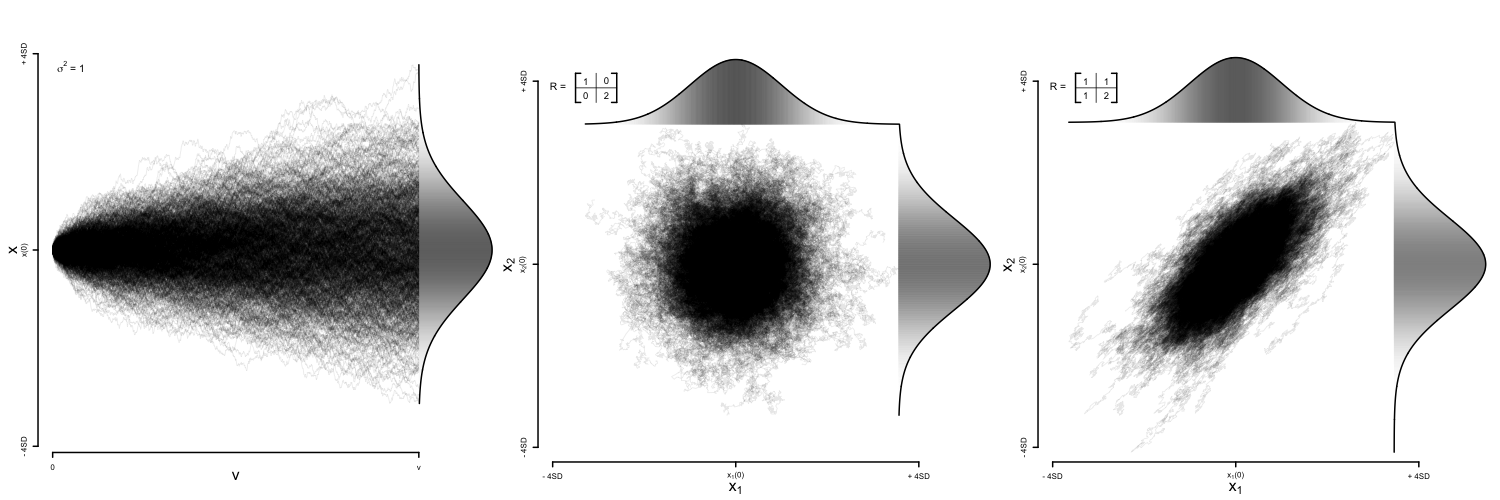
\includegraphics[width=160mm]{figures/unibivariateBMseed24.png}
\caption[Visualizing Brownian Motion in One and Two Dimensions]{Visualizing Brownian motion in one and two dimensions. In a), we see 1,000 realizations from a uvBM process with rate given by $\sigma^2$ = 1 over branch length $v$. The vertical axis is centered on the starting value of the process, $x(0)$, with bounds +/- 4 standard deviations of the normal distribution describing the ending state. This normal distribution is drawn in the right margin, with shade proportional to probability density at each value $x$. In b), we see this process generalized to two dimensions for characters $x_1$ and $x_2$, with rate matrix $R$ in the upper left corner. As off-diagonal elements of $R$ were set to 0, this is equivalent to a uvBM process of two independent characters. In c), we observe realizations from a bivariate Brownian motion where off-diagonals are non-zero -- here, the correlation between characters is $\frac{1}{\sqrt{2}} \approx 0.71$. 
\label{overflow}
\label{fig:univBM}
}
\end{figure*}

\begin{figure}[t]
\centering
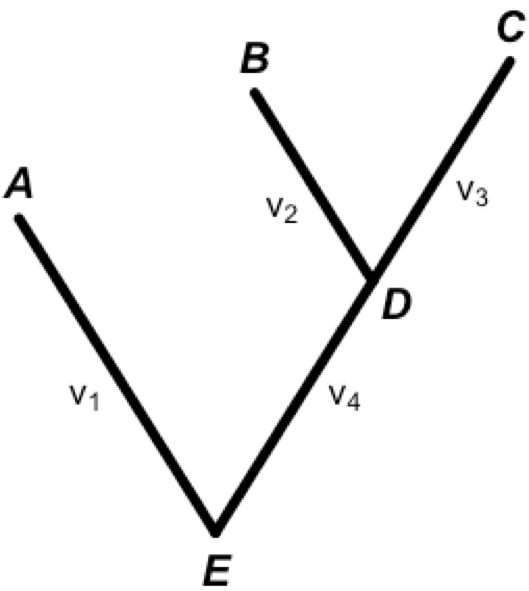
\includegraphics[width=50mm]{figures/simple3tiptree.png}
\caption[A Simple Rooted Tree with Three Tips]{A 3-tip, rooted phylogenetic tree with branches $\{v_1, v_2, v_2, v_4\}$ and nodes $\{A, B, C, D, E\}$ labeled. 
\label{overflow}
\label{fig:simpleTree}
}
\end{figure}

\begin{figure}[th]
\centering
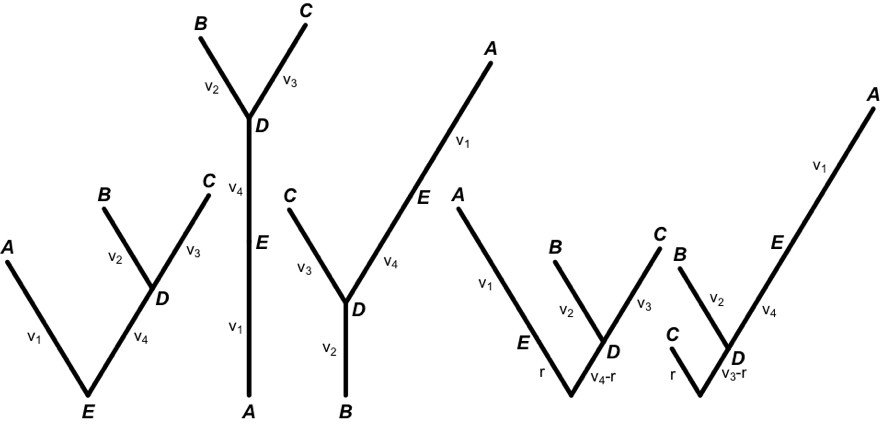
\includegraphics[width=85mm]{figures/identicalLikelihoods.png}
\caption[Visualizing the Pulley Principle Under mvBM]{Given character data at $\{A, B, C\}$ and labeled edge lengths, all of the above trees have identical likelihoods, marginalizing over unobserved states. \label{overflow}
\label{fig:pulleyPrinciple}
}
\end{figure}

\begin{figure*}[h]
\centering
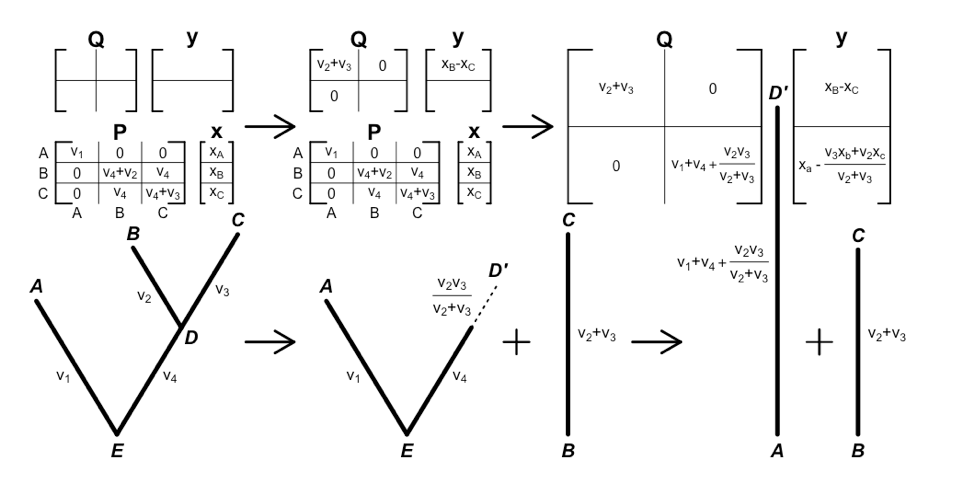
\includegraphics[width=160mm]{figures/pruningAlgorithm.png}
\caption[The Pruning Algorithm Applied to a Tree]{The pruning algorithm applied to the tree in Figure \ref{fig:simpleTree} and used to construct matrix $Q = CPC^T$ and vector $y = Cx$. 
\label{overflow}
\label{fig:pruningAlgorithm}
}
\end{figure*}

\begin{figure*}[h]
\centering
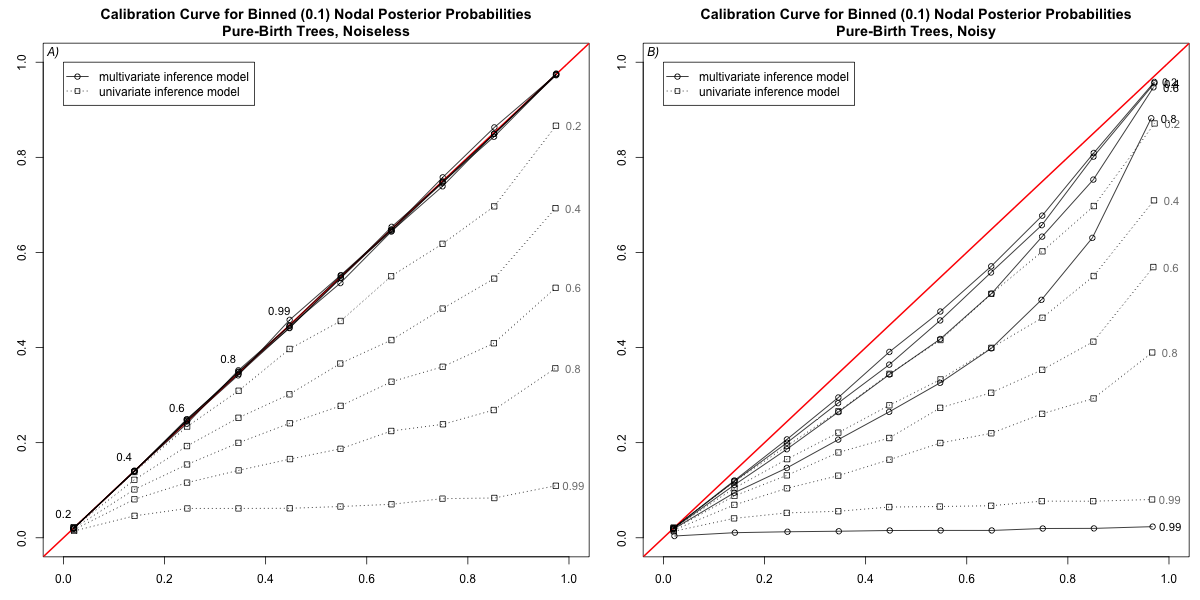
\includegraphics[width=\textwidth]{figures/calibrationCurvePBT.png}
\caption[Calibration Curves for the Brownian Motion Simulation Study, Idealized Conditions]{Calibration curves for the analyses of pure-birth trees, averaged across replicates and trait numbers. Solid lines represent inference under a multivariate Brownian motion model, with individual lines representing the strength of correlations between traits in the rate matrix. Dotted lines represent calibration curves under the univariate inferential model, with correlation strengths labeled. A line through the origin with a slope of 1 represents perfect calibration. The horizontal axis marks the average probability of bipartitions falling within bins of 0.1 width, and the vertical axis marks the frequency with which those bipartitions appeared in their corresponding data-generating trees. The left plot a) depicts analyses where no noise was added to the tip means; the right plot b) shows analyses where tip values were perturbed by added noise (described in text).
\label{overflow}
\label{fig:calibrationCurvePBT}
}
\end{figure*}

\begin{figure*}[h]
\centering
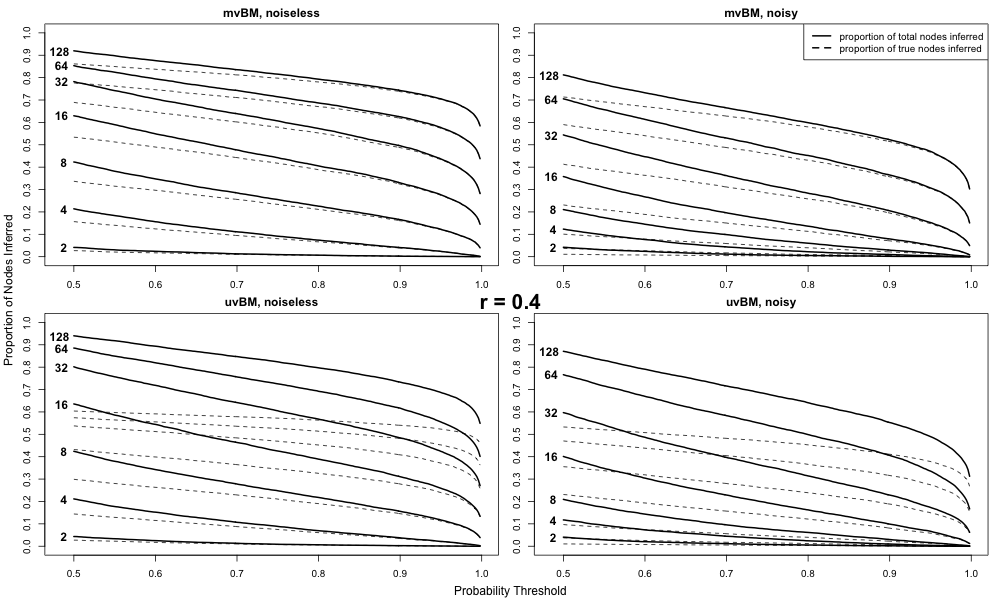
\includegraphics[width=160mm]{figures/CARcurvesPBT.png}
%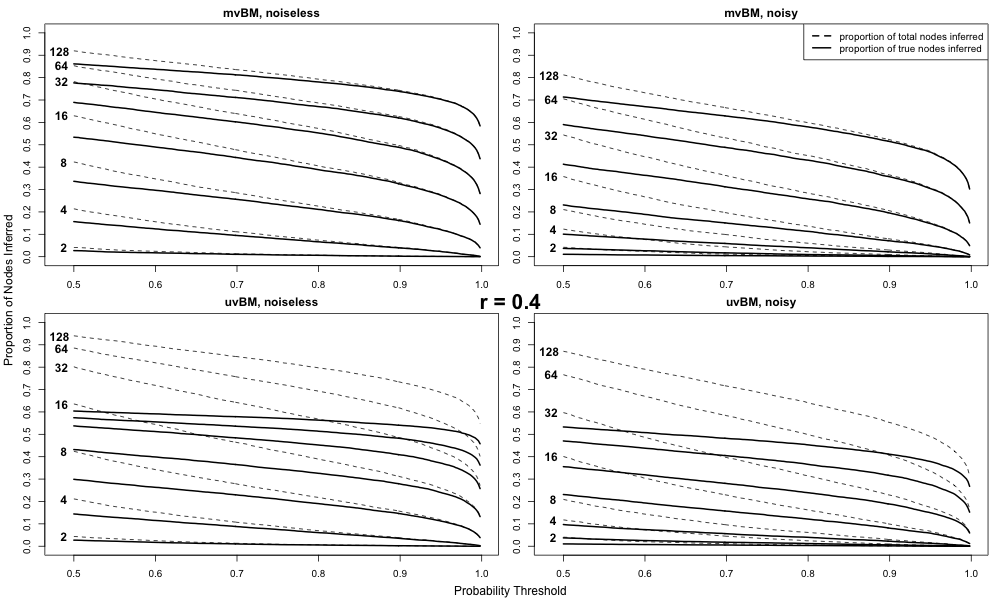
\includegraphics[width=160mm]{figures/CARcurvesPBT_swapLineStyle.png}
\caption[Cumulative Average Resolution Curves for the Brownian Motion Simulation Study, Idealized Conditions]{Cumulative Average Resolution (CAR) curves for analyses of character alignments simulated under multivariate Brownian motion on pure-birth trees. Here, we see curves corresponding to moderate correlation structure (correlations of 0.4 in the multivariate Brownian motion rate matrix); plots for other correlation structure conditions can be seen in Supplemental Figure 1. The vertical axis represents the proportion of nodes occurring above some probability threshold, shown on the horizontal axis, averaged across replicates for each trait number. Trait numbers corresponding to each curve appear in the left portion of the figure. Solid lines correspond to the ratio of the total number of nodes inferred above each probability threshold to the maximum number of nodes appearing in the true, unrooted tree, while dashed lines represent only those inferred nodes which are actually present in the true, unrooted tree. 
\label{overflow}
\label{fig:carCurvePBT}
}
\end{figure*}

\begin{figure*}[h]
\centering
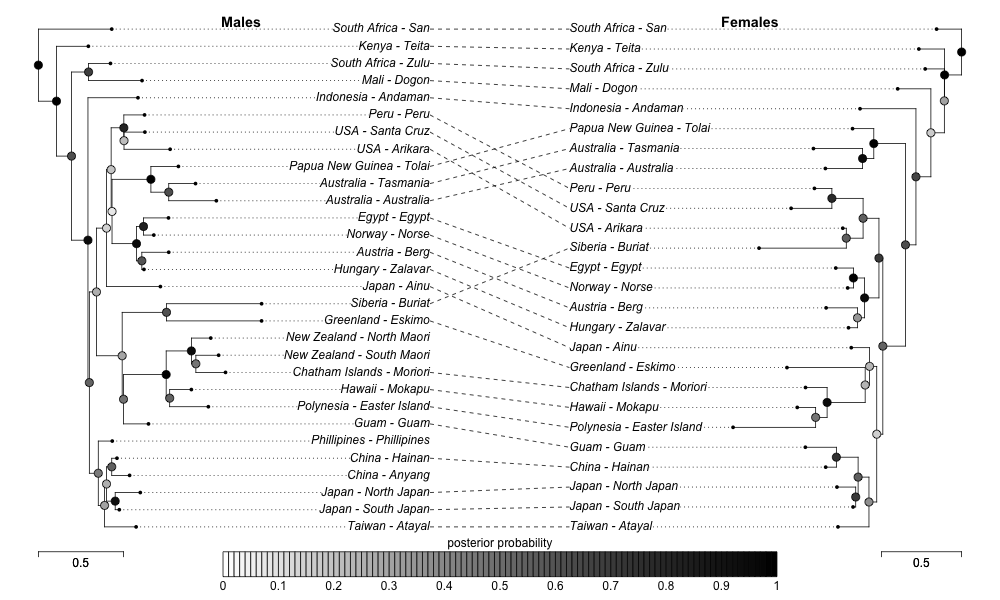
\includegraphics[width=160mm]{figures/howellsTreesMF.png}
\caption[Maximum Clade Credibility Trees for Empirical Analyses of Howells' Data]{Two Maximum-Clade Credibility (MCC) trees are shown, each computed from MCMC output of Howells’ craniometric measurements, with the left corresponding to population means of individuals identified as male by Howells, and the right identified female. Nodes have been rotated in each to minimize the mismatch of vertical tip ordering using the \texttt{cophylo()} function in Phytools \citep{revellPhytoolsPackagePhylogenetic2012}. Trees have been rooted with the “South Africa - Sān” population serving as the outgroup for viewing convenience. Posterior probabilities at each internal node are represented by grayscale circles, with key shown. Scale bars are included for each tree to allow visual comparison of branch lengths in units of average within-population differentiation (a single unit of branch length corresponds morphological evolution comparable to the average amount of variation within each tip population; i.e., a draw from the same multivariate normal distribution).
\label{overflow}
\label{fig:mccCophylo}
}
\end{figure*}

\begin{figure*}[h]
\centering
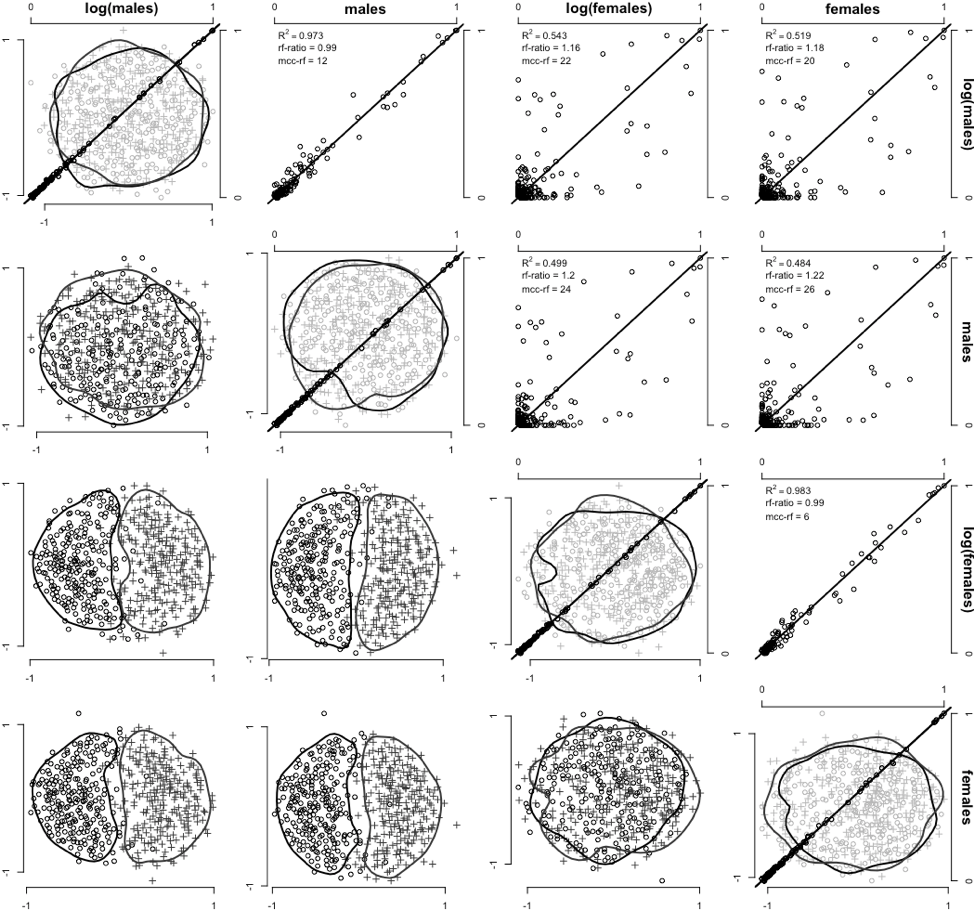
\includegraphics[width=140mm]{figures/sensitivityHowells.png}
%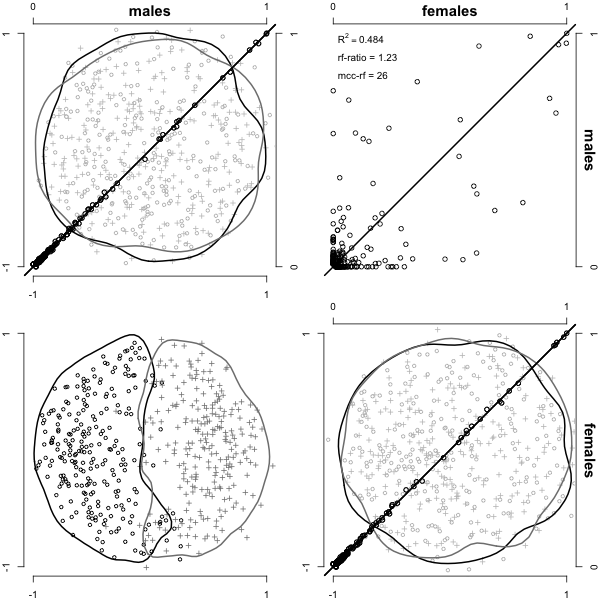
\includegraphics[width=140mm]{figures/sensitivityHowells_2x2.png}
\caption[Visualizing Sensitivity to Researcher Degrees of Freedom in Analysis of Howells' Data]{Sensitivity to choice of dataset (male vs. female) and model (arithmetic vs. geometric mvBM) is compared through multidimensional scaling (MDS) and compare-trees plots. The former find a set of 2-dimensional coordinates whose distances are closest to a distance matrix provided, in this case a matrix of pairwise RF distances between samples from the MCMC output of analyses represented by the rows and columns. Here, we used 500 trees from each analysis to compute MDS coordinates, but for ease of viewing only plotted 250 points from each analysis. Circles represent the row analysis and + signs the column analysis, with 95\% contour envelopes drawn. The latter compare posterior probabilities for the same bipartition (with probability threshold equal to or greater than 0.01) between each analysis, with complete agreement between analyses finding points that fall along the 1-to-1 line. Diagonals represent both types of plot overlain for two independent chains of the same analysis.\label{overflow}
\label{sensitivitySexGeom}
}
\end{figure*}

\begin{figure*}[h]
\centering
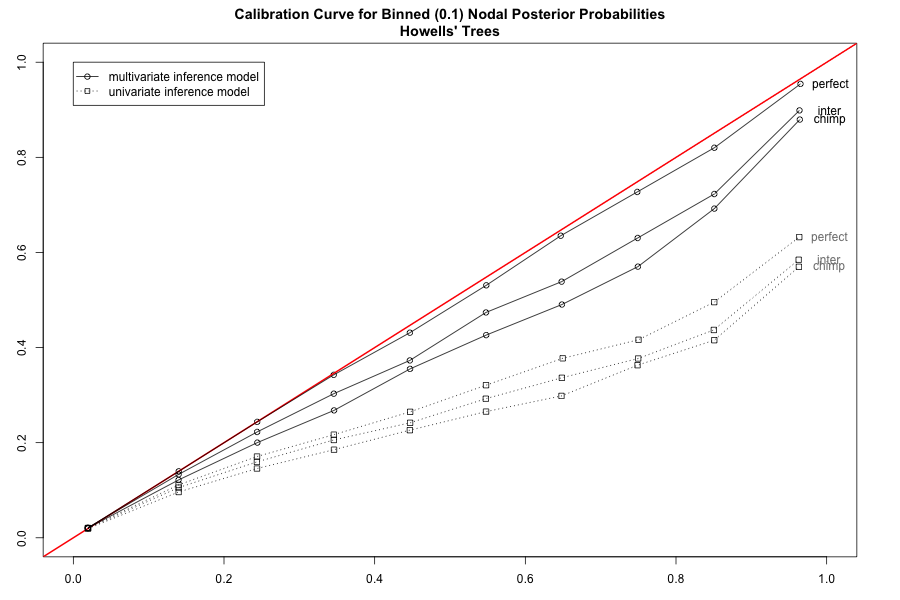
\includegraphics[width=120mm]{figures/calibrationCurveHowells.png}
\caption[Calibration Curves for the Brownian Motion Simulation Study, Empirically Parameterized Conditions]{Calibration curves for the analyses of Howells’ simulations, with rate matrix specification conditions labeled. See main text and caption for Figure \ref{fig:calibrationCurvePBT} for further information.
\label{overflow}
\label{fig:calibrationCurveHowells}
}
\end{figure*}

\begin{figure*}[h]
\centering
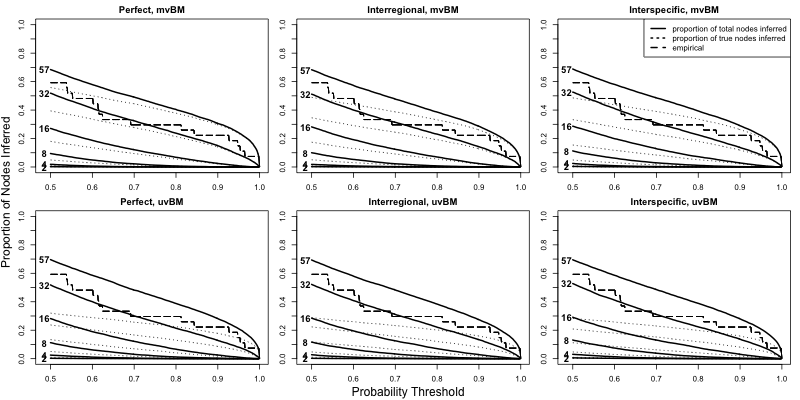
\includegraphics[width=160mm]{figures/CARcurvesHowells_BW.png}
\caption[Cumulative Average Resolution Curves for the Brownian Motion Simulation Study, Empirically Parameterized Conditions]{CAR curves for the analyses of Howells’ simulations, with rate matrix specification conditions labeled. A stairstep-like line for the arithmetic analysis of Howells’ 57 craniometric measurements collected on individuals estimated to be male is overlain, though no qualitative difference in the location or shape of this curve across different datasets or models could be seen. See main text and caption for Figure \ref{fig:carCurvePBT} for further information.
\label{overflow}
\label{fig:carCurveHowells}
}
\end{figure*}

\clearpage

\section{Tables}

% latex table generated in R 3.6.2 by xtable 1.8-4 package
% Wed Sep 30 15:25:16 2020
\begin{longtable}{rrrr}
  \hline
 & Females & Males & Total \\ 
  \hline
Japan - Ainu &  38 &  48 &  86 \\ 
  Indonesia - Andaman &  35 &  35 &  70 \\ 
  China - Anyang &   0 &  42 &  42 \\ 
  USA - Arikara &  27 &  42 &  69 \\ 
  Taiwan - Atayal &  18 &  29 &  47 \\ 
  Australia - Australia &  49 &  52 & 101 \\ 
  Austria - Berg &  53 &  56 & 109 \\ 
  Siberia - Buriat &  54 &  55 & 109 \\ 
  South Africa - Sān &  49 &  41 &  90 \\ 
  Mali - Dogon &  52 &  47 &  99 \\ 
  Polynesia - Easter Island &  37 &  49 &  86 \\ 
  Egypt - Egypt &  53 &  58 & 111 \\ 
  Greenland - Eskimo &  55 &  53 & 108 \\ 
  Guam - Guam &  27 &  30 &  57 \\ 
  China - Hainan &  38 &  45 &  83 \\ 
  Hawaii - Mokapu &  49 &  51 & 100 \\ 
  Chatham Islands - Moriori &  51 &  57 & 108 \\ 
  Japan - North Japan &  32 &  55 &  87 \\ 
  New Zealand - North Maori &   0 &  10 &  10 \\ 
  Norway - Norse &  55 &  55 & 110 \\ 
  Peru - Peru &  55 &  55 & 110 \\ 
  Phillipines - Phillipines &   0 &  50 &  50 \\ 
  Japan - South Japan &  41 &  50 &  91 \\ 
  New Zealand - South Maori &   0 &  10 &  10 \\ 
  USA - Santa Cruz &  51 &  51 & 102 \\ 
  Australia - Tasmania &  42 &  45 &  87 \\ 
  Kenya - Teita &  50 &  33 &  83 \\ 
  Papua New Guinea - Tolai &  54 &  56 & 110 \\ 
  Hungary - Zalavar &  45 &  53 &  98 \\ 
  South Africa - Zulu &  46 &  55 & 101 \\ 
   \hline
\hline
\caption[Composition of Linear Measurement Data Used in Empirical Analysis]{A table detailing the composition of Howells' linear measurement dataset used in 
                                            our empirical analysis. Elements of the table represent numbers of individuals in each 
                                            population corresponding to each 
                                            estimated column sex. Further details regarding the nature of this sample can be found in \citep{howellsWhoWhoSkulls1995}.} 
\label{tab:howellsDataComposition}
\end{longtable}


\clearpage
\twocolumn
%\nocite{*}
\bibliographystyle{apalike}
{
\footnotesize
\bibliography{sysbio_paper_references.bib}
}

\end{document}
